

\documentclass[a4paper]{article}

\usepackage[utf8]{inputenc}
\usepackage{graphicx}


\title{Mi test de un articulo de latex}
\author{Roosevelt Garc\'ia Paredes}

\begin{document}
\maketitle


\section{Introduccion}
Es una cadena de presentación de la introducción del artículo, en la cual se describe el contenido del mismo y se da un contexto general de lo que se va a tratar.

\subsection{Background}
% \includegraphics{anexos/Latex-Parte VI.png}[height=5cm]

\begin{figure}[ht]
    \centering
    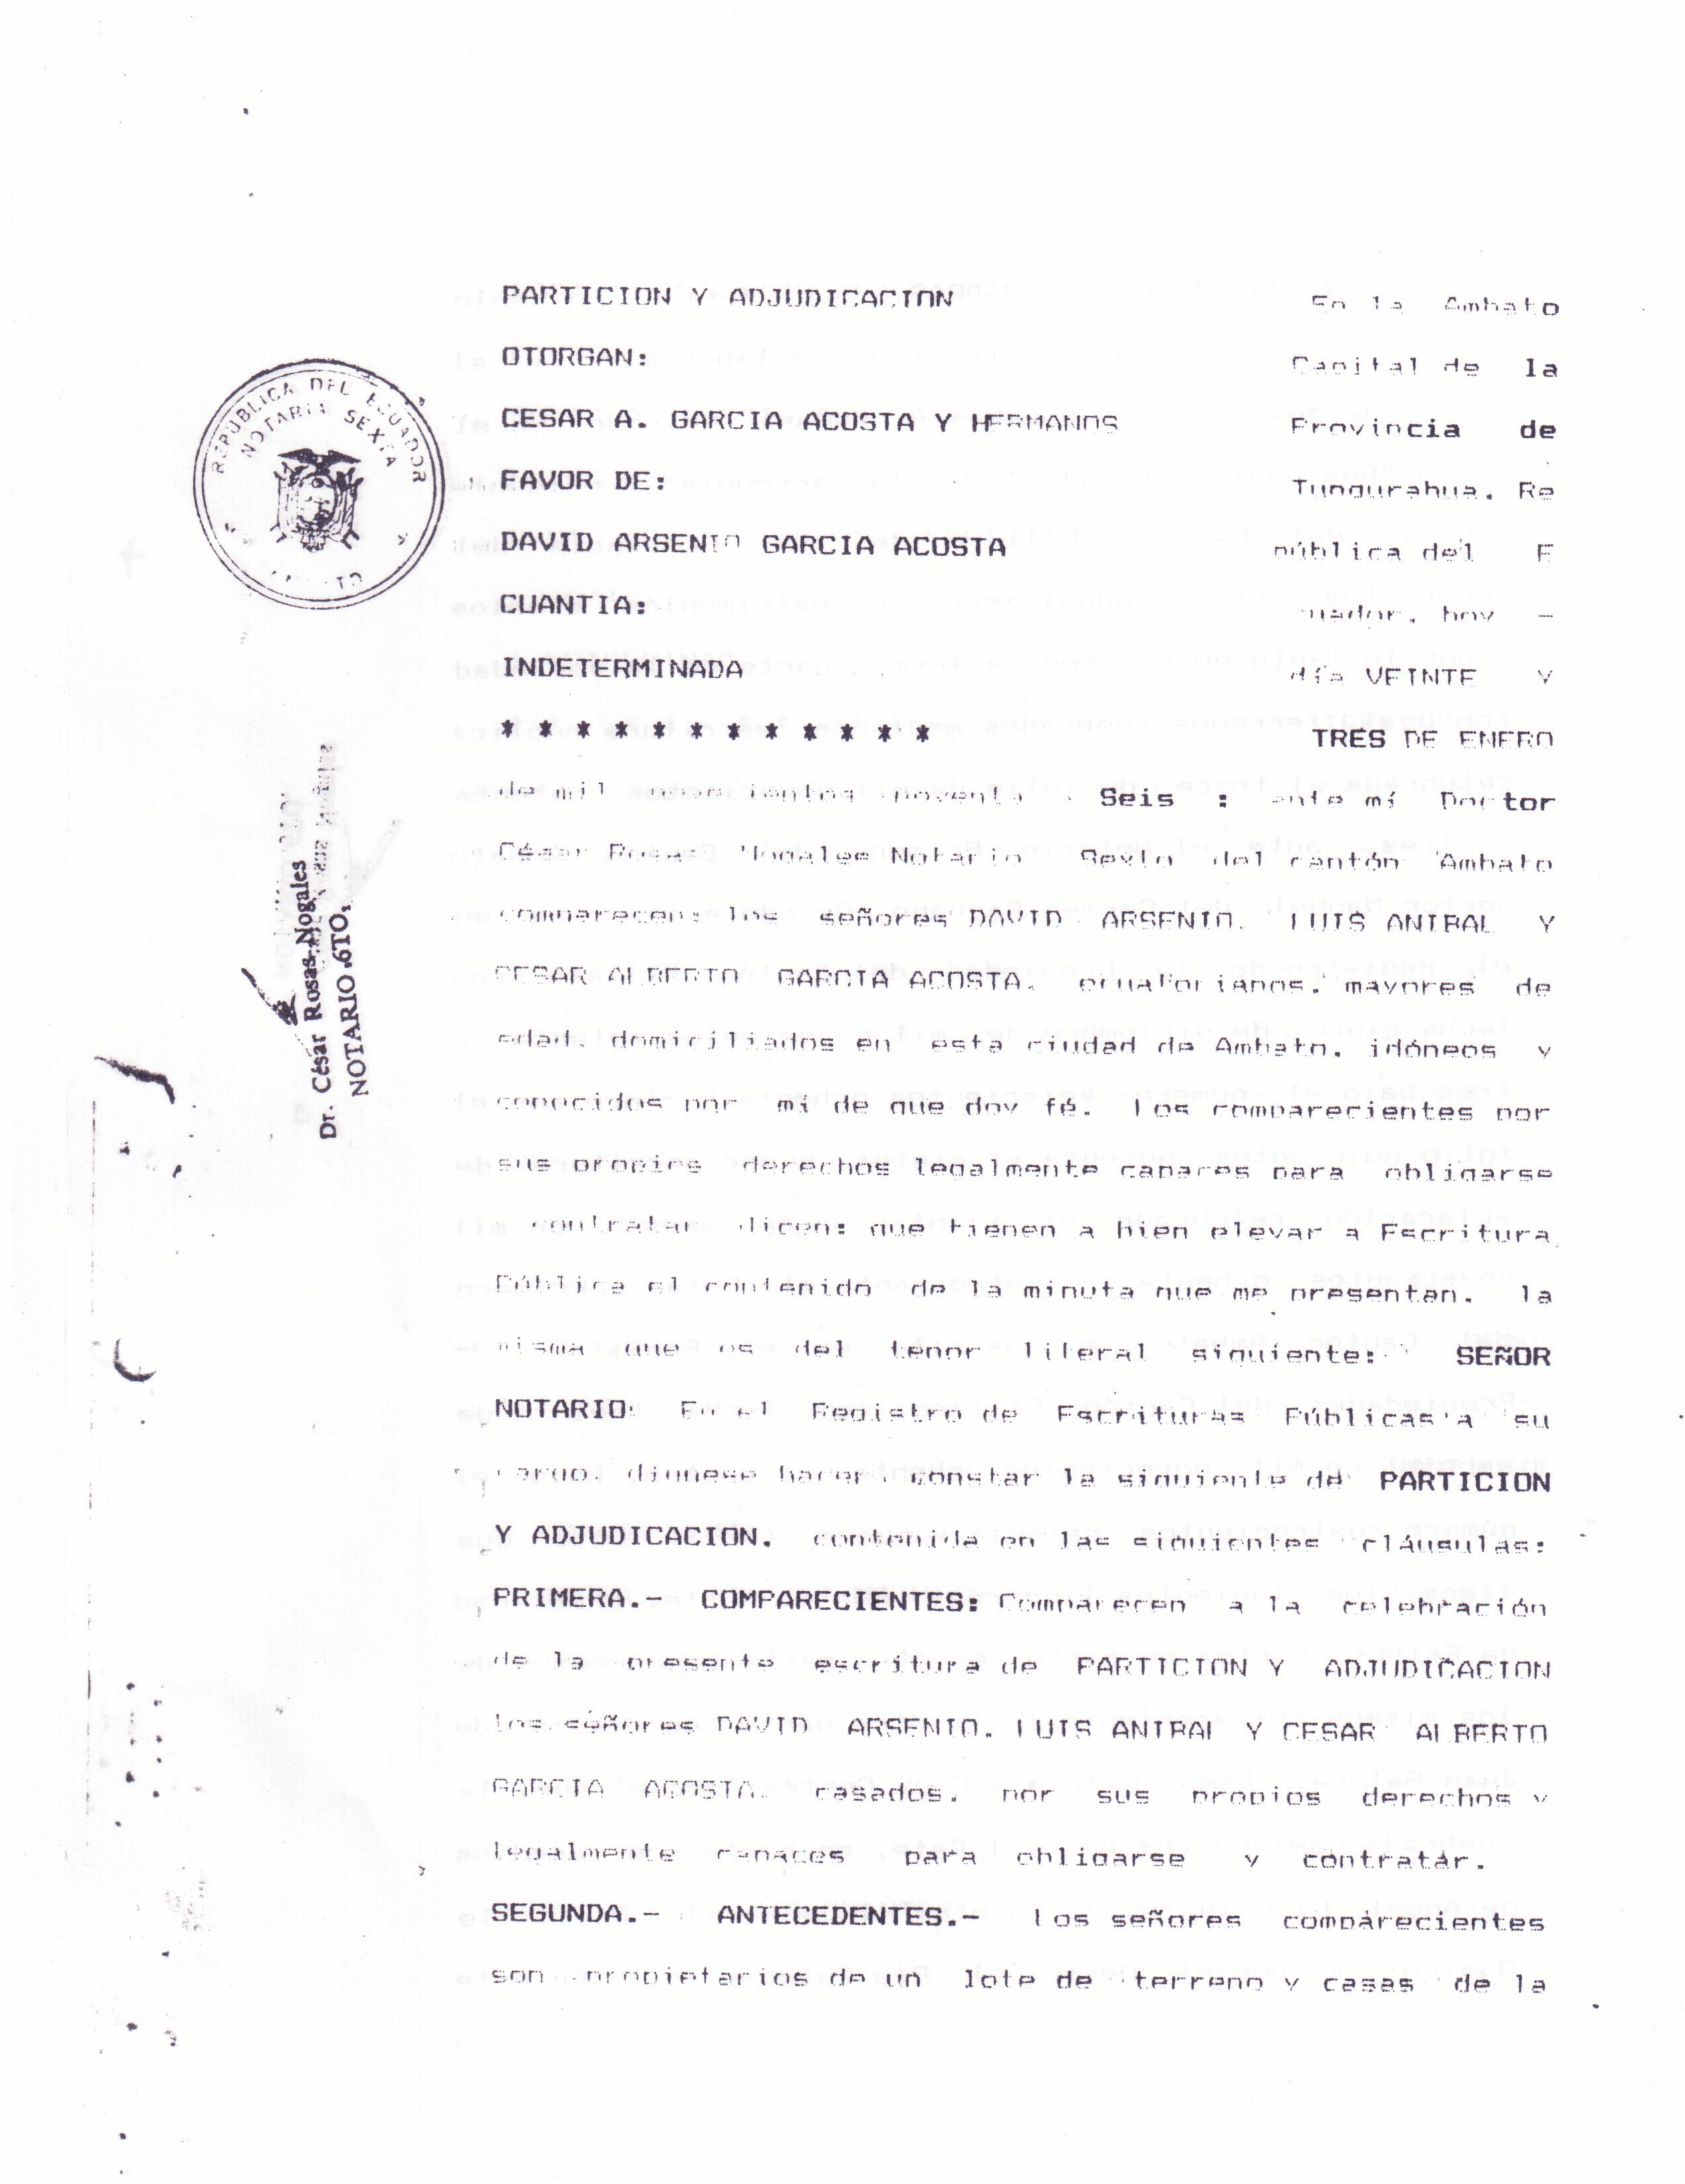
\includegraphics[height=5cm]{anexos/img1.jpg}
    \caption{Página del concepto de análisis}
    \label{fig:Pagina1}    
\end{figure}
Es un nuevo texto de mas de  una linea cmo  puedeo manejar \\
esto kassakakakaaskakjasdkldkasdkasdasas\\
sienpre es asi \\

Listo \\ Hay que colocar el nuevo parrafo

\begin{figure}[ht]
    \centering
    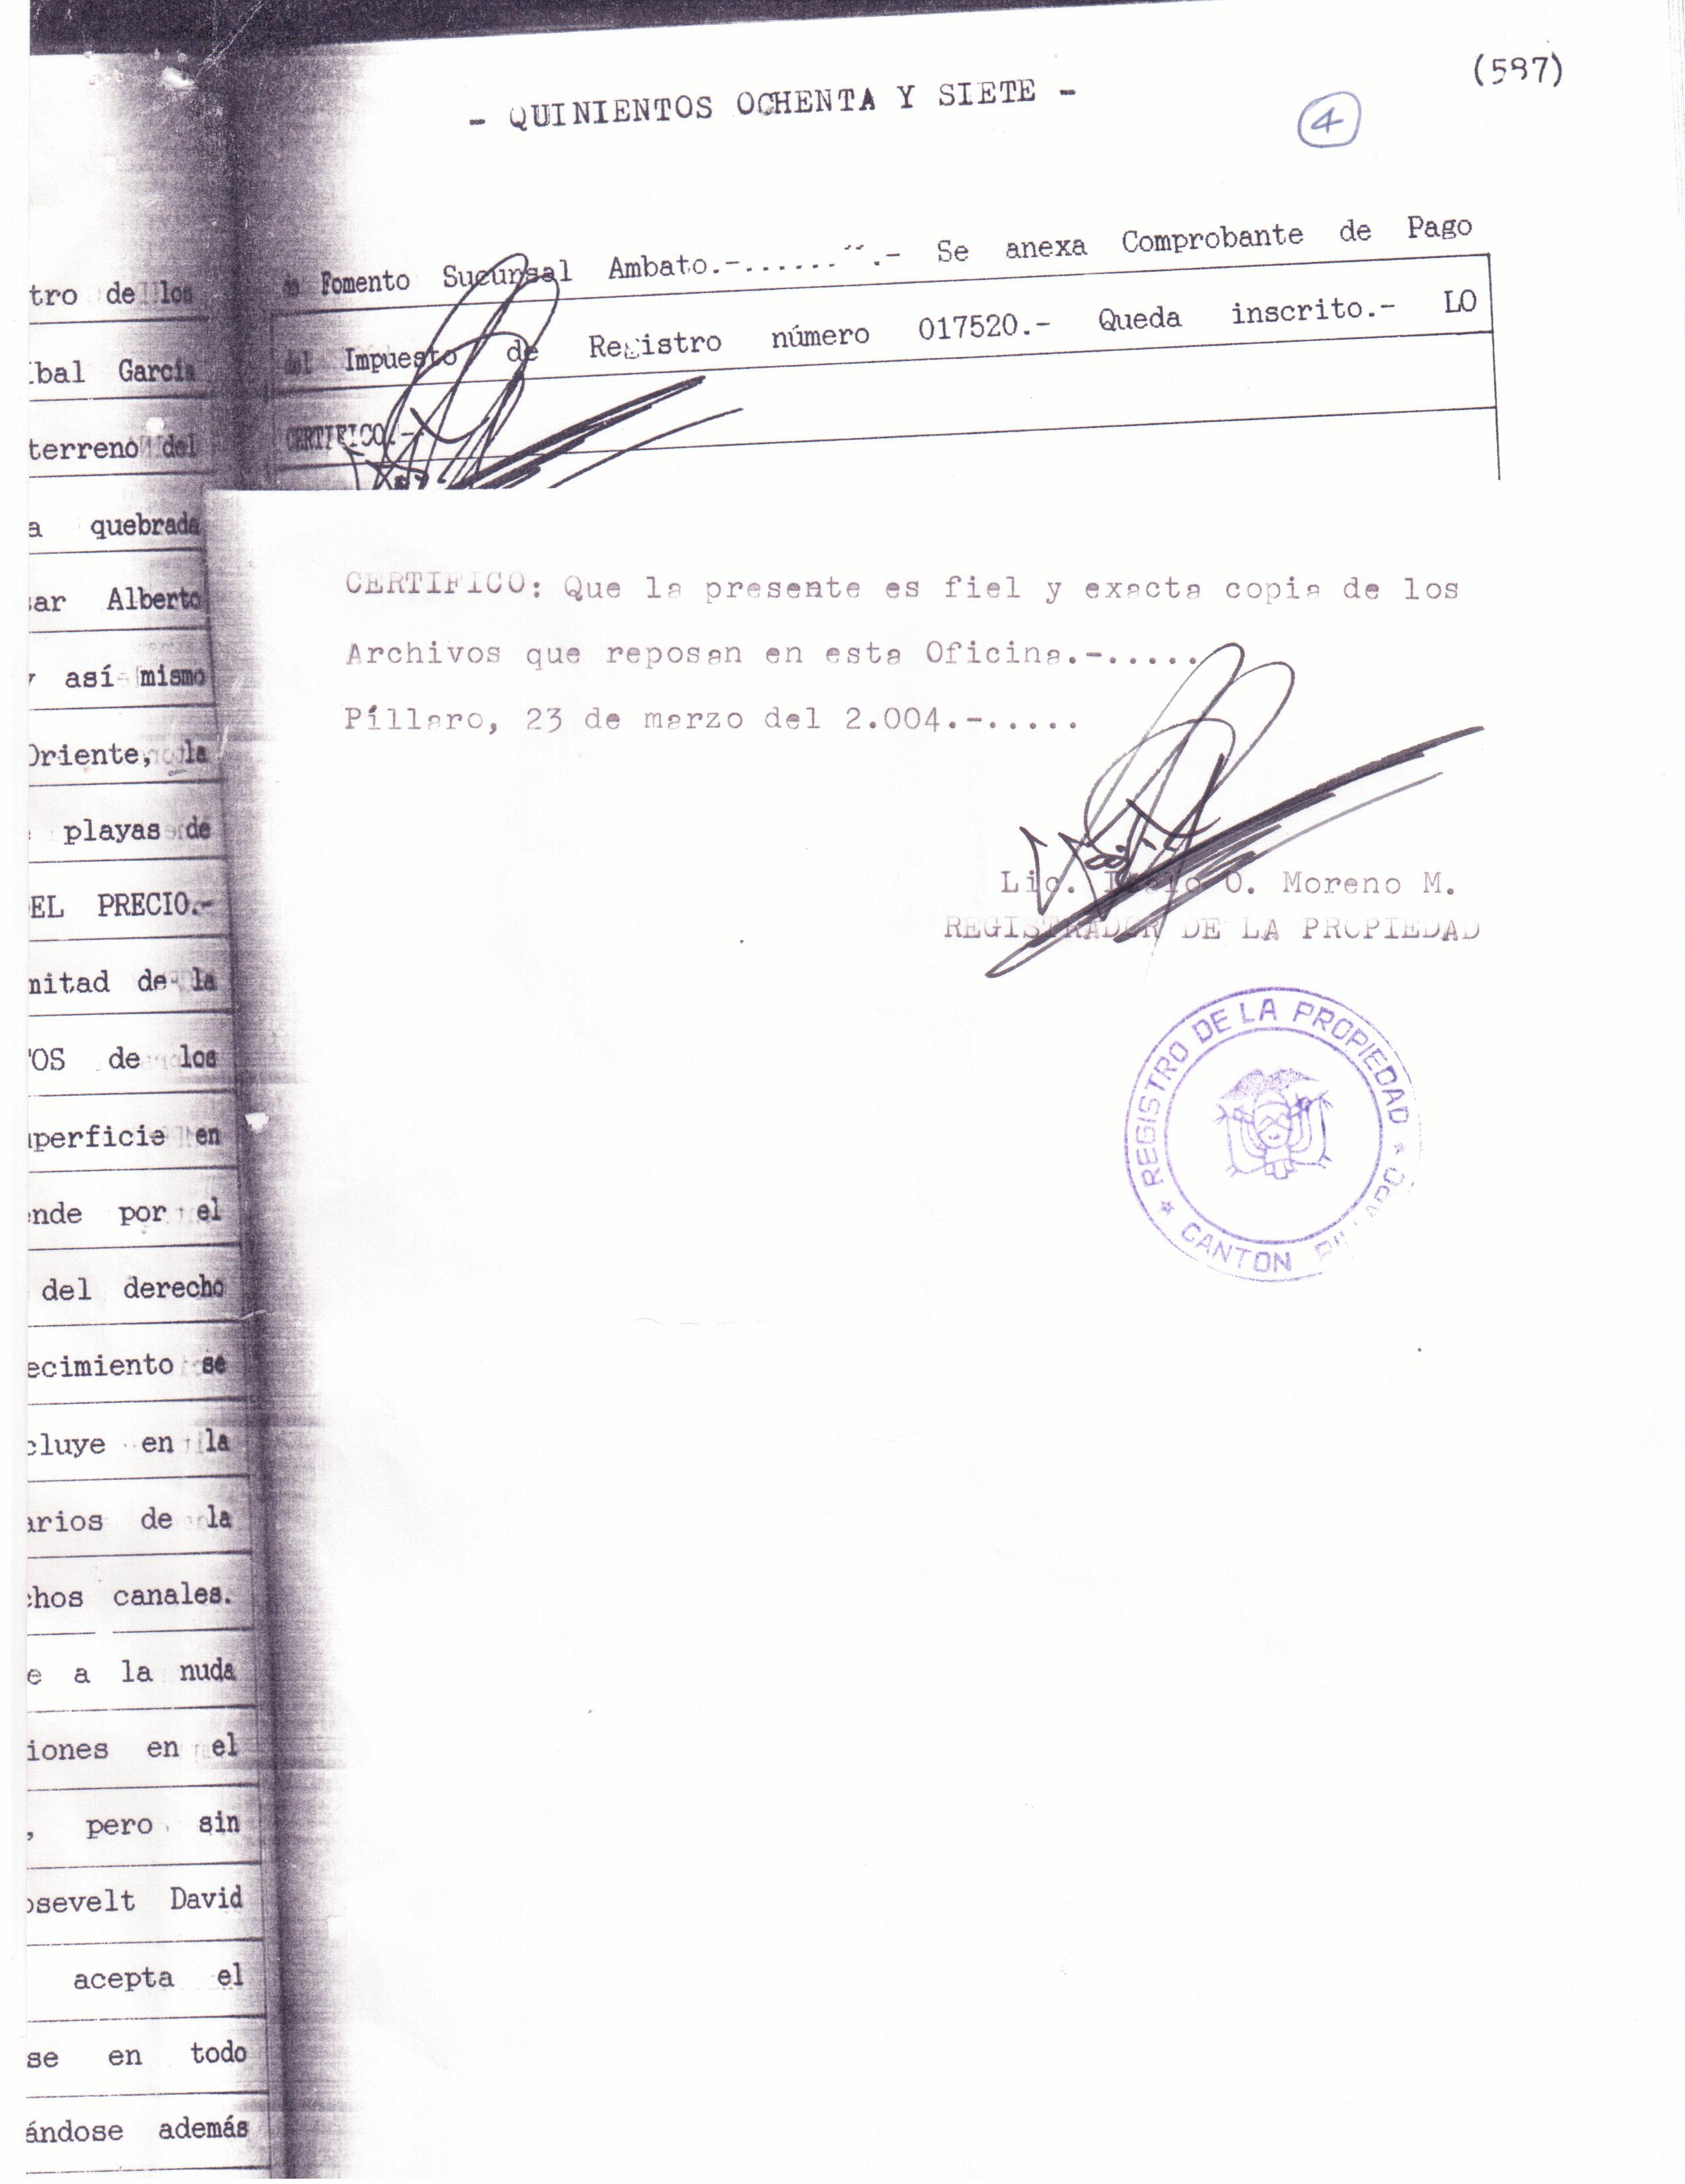
\includegraphics[height=5cm]{anexos/img2.jpg}
    \caption{Página 2, desarrollo del concepto de análisis}
    \label{fig:Pagina2}    
\end{figure}

\section{Analisis}
$ Ambato= \beta * n ^{2} + \gamma $

\end{document}